\documentclass[a4paper]{scrartcl}

\usepackage[utf8]{inputenc}
\usepackage{enumitem}
\usepackage{tikz}
\usepackage{amsmath}
\usepackage{amssymb}

\usepackage{anysize}
\usepackage{multirow}
\usepackage{verbatim}
\usepackage{lscape}
\usepackage{graphicx}

\marginsize{2.0cm}{2cm}{2.5cm}{2.5cm}

\author{Gruppe 6}

\title{\textbf{VerteilteWebInf Hausaufgabe 11}}
\date{\today}


\begin{document}
\maketitle

\section*{Aufgabe 1}
\begin{enumerate}[label=\alph*)]

\item Zur Verwendung des RSA-Verfahrens wird hier ein öffentlicher Schlüsselverwalter vorausgesetzt, sodass sich der Client den Public Key des Servers von dort holen kann. \\
Dann sendet der Client seinen eigenen Public Key $ E_C $ mit dem Public Key des Servers verschlüsselt an den Server. So ist sichergestellt, dass nur der Server mit seinem Private Key $ D_S $ den Public Key des Clients entschlüsseln kann. \\
Nun können Nachrichten versendet werden. Dazu signiert der Client zuerst seine Nachricht mit seinem Private Key $ D_C $, damit sichergestellt ist, dass nur er diese Information verfasst haben kann. Damit diese Nachricht wiederum nur der Server lesen kann, wird diese noch mit dem Public Key $ E_S $ des Servers verschlüsselt. Der Server kann diese Nachricht entschlüsseln indem er zuerst seinen Private Key darauf anwendet und dann den Public Key des Clients. Analog kann eine Nachrichtenübermittlung in die entgegen gesetzte Richtung stattfinden. 

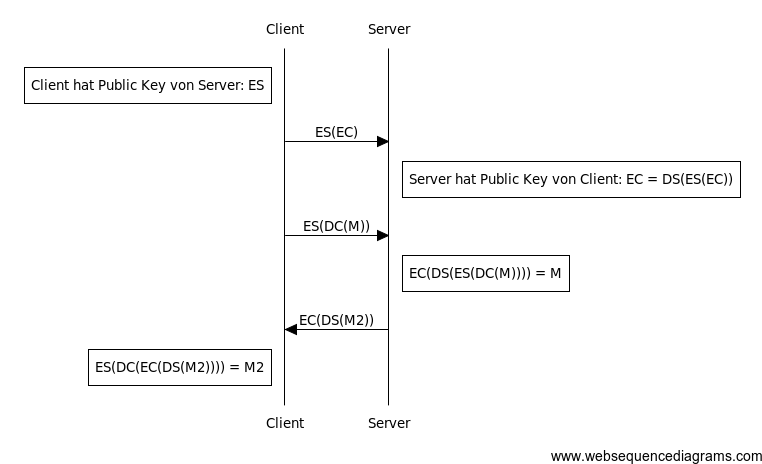
\includegraphics[width=15cm]{sequenzdiagramm.png}

\item Ja, das System ist sicher gegenüber Man-in-the-middle-Attacken. Die Korrektheit des öffentlichen Schlüssels des Servers wird über einen öffentlichen Schlüsselverwalter vorausgesetzt. Bei der Mitteilung des Schlüssels des Clients kann diesen nur der Server mit seinem Private Key entschlüsseln. Somit kennt nur der Server den Public Key des Clients und kein Man-in-the-Middle kann diesen abfangen, um das Gespräch zwischen den beiden Gesprächspartnern zu simulieren. 

\item Funktionsweise einer PKI: Digitale Zertifikate stellen die Echtheit der öffentlichen Schlüssel sicher. Diese Zertifikate sind durch eine digitale Signatur geschätzt und somit ist sichergestellt, dass sie von einer entsprechenden Zertifizierungsstelle stammen. \\
Nötig ist zudem eine Zertifikatsstatusprüfung, sodass sichergestellt ist, dass das Zertifikat beispielsweise nicht zurückgezogen wurde. Dies kann durch Black-Lists (auf denen alle zurückgezogenen Zertifikate vermerkt sind) oder White-Lists (auf denen alle gültigen Zertifikate vermerkt sind) realisiert werden. \\
Eine PKI stellt somit die Zertifikate mit den Public Keys und eine Möglichkeit der Überprüfung derer zur Verfügung. 
\\
Authentifizierung an einem Beispiel: Die PKI besitzt nur beispielweise den Public Key des Servers und der Client möchte diesen erfahren. Dann sendet der Client eine Anfrage an die PKI und erhält nun ein Zertifikat, das mit dem Private Key des Ausstellers verschlüsselt wurde. Zum Entschlüsseln ist nun der Public Key des Zertifikatausstellers zu verwenden, der rekursiv aufgelöst werden kann bis man bei einer sogenannten Root-CA angekommen ist, von der einem der Public Key bekannt ist. In dem angeforderten Zertifikat befindet sich nun der gesuchte Public Key des Servers und der Client hat sichergestellt, dass es der richtige ist. 

\item Felder des X.509-Zertifikats von "devschlichter.in.tum.de"
\begin{itemize}
\item Allgemeine Informationen über das Zertifikat: Zertifikatsinformationen: Version (3), Seriennummer, Zertifikatsunterzeichnungs-Algorithmus (PKCS \#1 SHA-1 mit RSA-Verschlüsselung), Aussteller (TUM).\\
Diese Informationen sind nötig, damit das Zertifikat eindeutig gelesen werden kann, es sind also Verwaltungsinformationen.
\item Validität: Hier ist der Gültigkeitszeitraum vermerkt. So sind die Zertifikate nur begrenzt gültig und müssen bei Änderungen nicht zurückgezogen werden.
\item Inhaber: Zur Identifikation sind hier die Daten (Name, E-Mail, Ort, Land, Organisation) vermerkt.
\item Angaben zum öffentlichen Schlüssel des Inhabers: Angabe des Algorithmus des Inhabers und dessen öffentlicher Schlüssel
\item Nun folgen mögliche Erweiterungen, um genauere Informationen mitzuteilen (z.B. Alternativ-Namen des Zertifikatsgegenstands)
\item Signatur des Zertifikats mit Angabe des verwendeten Algorithmus zur Wahrung des Authentizität
\end{itemize}

\item Damit nicht eine Zertifizierungsautorität alle Zertifikate verwalten muss, kann eine Zertifikatshierarchie aufgebaut werden. Dies dient also der dezentralen Organisation. Ein Beispiel: \\
devschlichter.in.tum.de $ \rightarrow $ Zertifizierungsstelle der TUM $ \rightarrow $ DFN-Verein PCA Global-G01 $ \rightarrow $ Deutsche Telekom Root CA 2


\end{enumerate}


\section*{Aufgabe 2}
b) Nein, sie sind keine Pipeline-Breaker.\\
\textit{Threshold}: Hier können alle Tupel die unter dem berechneten Threshold liegen bereits weitergereicht werden.\\
\textit{NRA}: Wenn hier ein Ergebnis feststeht und keine Ergebnisse mit niedrigeren Kosten existieren, kann das Tupel weitergereicht werden. 







\end{document}


